\chapter{Methodology}

\section{Task}
For a short text segment, $T = \{t_1, t_2, ..., t_n\}$ where $t_i$ is defined as a token, classify if the sequence of tokens $T$ is a complaint or not.

\section{Data and pre-processing}
The data used for the experiments is from Twitter. Twitter provides a good representation of social media text due to the direct connection consumers have with organisations and brands as well as the ability to express oneself \cite{preotiuc-pietro_automatically_2019}. **Add content on why Twitter**
\newline \newline
The data set created by \cite{preotiuc-pietro_automatically_2019} and further used by \cite{jin_complaint_2020} is utilised for this project. The original process for collection and annotation employed by them is breifly described below. The particular version \footnote{The data can be found here - https://archive.org/details/complaint\_severity\_data} used for the experiments is the one enhanced by \cite{jinModelingSeverityComplaints2021} with the addition of labels for the severity of complaints. These additional labels are not used for the experiments in this project.
\subsection{Domains and organisations}
A cross-industry representative collection of 93 customer service handles of organisations on Twitter were identified manually. These handles were then categorised into 9 domains based on their industry type. Since an organisation could have business activities across domains, the assigned domain was based on the products or services receiving the most number of complaints. All the domains used in the experiments are listed in Table \ref{tab: domains}. 
\begin{table}[ht]
    \captionsetup{font=small}
    \centering
    \begin{tabularx}{\textwidth}{|X|c|c|c|}
    \hline
    \rowcolor[gray]{0.7}
    \textbf{Domains} & \textbf{Complaints} & \textbf{Non-Complaints} & \textbf{Total Tweets}\\
    \hline
    Food \& Beverage & 95 \small{(73\%)} & 35 \small{(27\%)} & 130 \small{(7\%)}\\
    \rowcolor[gray]{0.9}
    Apparel & 141 \small{(55\%)} & 117 \small{(45\%)} & 258 \small{(13\%)}\\
    Retail & 124 \small{(62\%)}& 75 \small{(38\%)} & 199 \small{(10\%)}\\
    \rowcolor[gray]{0.9}
    Cars & 67 \small{(73\%)} & 25 \small{(27\%)}  & 92 \small{(4\%)} \\
    Services  & 207 \small{(61\%)} & 130 \small{(39\%)}  & 337 \small{(17\%)} \\
    \rowcolor[gray]{0.9}
    Software \& Online Services & 189 \small{(65\%)} & 103 \small{(35\%)}  & 292 \small{(15\%)} \\
    Transport & 139 \small{(56\%)} & 109 \small{(44\%)}  & 248 \small{(12\%)} \\
    \rowcolor[gray]{0.9}
    Electronics & 174 \small{(61\%)} & 112 \small{(39\%)}  & 286 \small{(15\%)} \\
    Other & 96 \small{(79\%)} & 33 \small{(21\%)}  & 129 \small{(7\%)} \\
    \hline
    \rowcolor[gray]{0.9}
    \textbf{Total} & 1232 \small{(63\%)} & 739 \small{(37\%)}& 1971\\
    \hline
    \end{tabularx}
    \caption{The nine domains and the distribution of tweets that are complaints and those that are not. The percentages indicate how the splits are distributed.}    
    \label{tab: domains}
\end{table}  

\subsection{Data Extraction}
The data was extracted from Twitter via the Twitter API \footnote{https://developer.twitter.com/en}. The most recent 3,200 tweets at the time of the collection exercise were extracted and the original tweets to which the customer service handles responded were identified. Then, random sampling equally for each handle, 1,971 tweets were identified where there was a response from the support's handle. To ensure a more balanced and diverse dataset, 1,478 randomly sampled tweets were added to the dataset. 739 tweets were replies to other handles (outside the 93 identified) and the remaining 739 tweets were not addressed to any Twitter handle. Table \ref{tab: tweet_counts} shows the breakdown of the total population of the tweets dataset. Tweets were filtered for English using langid.py \cite{luiLangidPyOfftheshelf2012}. Retweets were excluded and all usernames and URLs were anonymised and replaced with placeholder tokens.
\begin{table}[ht]
    \captionsetup{font=small}
    \centering
    \begin{tabularx}{\textwidth}{|X|c|c|c|}
        \hline
        \rowcolor[gray]{0.7}
        \textbf{Extraction Criteria} & \textbf{Complaints} & \textbf{Non-Complaints} & \textbf{Total Tweets} \\
        \hline
        Addressed to and replied by the identified 93 customer service handles & 1239 \small{(63\%)}  & 739 \small{(37\%)}  & 1971 \small{(58\%)}  \\
        \hline
        Addressed to other customer service handles & 0 & 739 \small{(100\%)} & 739 \small{(21\%)}  \\
        \hline
        Not addressed to any Twitter handle & 0 & 739 \small{(100\%)} & 739 \small{(21\%)}  \\
        \hline    
        \rowcolor[gray]{0.9}
        Total & 1232 \small{(36\%)}  & 2217 \small{(64\%)}  & 3449 \\
        \hline
    \end{tabularx}
    \caption{Selection of tweets based on random sampling and where they have received replies when addressed to the 93 customer service handles combined with random sampled tweets that are addressed to other handles and tweets that are not addressed to any handle.}    
    \label{tab: tweet_counts}
\end{table}  

\subsection{Annotation}
The classification of the 1,971 tweets as complaints or not was carried out using a binary annotation task (complaint or not). Since tweets are concise and typically express a single idea, an entire tweet was classified as a complaint if it contained at least one speech act of complaining. To guide the annotation process, a complaint definition from \cite{olshtain_speechact_1987}, stating that a complaint portrays a situation that contradicts the writer's positive expectation was used. Two of the authors with extensive annotation experience in linguistics independently labelled the 1,971 tweets. They had substantial agreement \cite{artsteinInterCoderAgreementComputational2008} with Cohen's Kappa of $\kappa$ = 0.731. In the end, 1,232 tweets (63\%) and 739 tweets (37\%) were identified as complaints and non-complaints. Table \ref{tab: domains} gives the breakdown of the complaint and non-complaint tweets for each domain.

\section{Environment and models}

\subsection{Hardware}
The primary details of the enviornment used for the experiments are listed below. 
\begin{itemize}
    \item \textbf{CPU Count:} 8
    \item \textbf{Memory:} 45 GB
    \item \textbf{GPU Count:} 1
    \item \textbf{GPU Model:} NVIDIA RTX A4000
    \item \textbf{GPU Memory:} 16 GB
\end{itemize}

\subsection{Software}
For the experiments, the BERT transformer large language models along with a number of its variants are used to classify the tweets and compare the performance. The models are based on the \textit{transformers} library implementation from Hugging Face\footnote{https://huggingface.co/} along with the \textit{datasets} and \textit{evaluate} libraries. From scikit-learn\footnote{https://scikit-learn.org/stable/} the \textit{sklearn} library is used to generate the stratified splits for the nested cross-fold validation. The versions for each library are shown in the table \ref{tab: libs_used}.

\begin{table}[ht]
    \captionsetup{font=small}
    \centering
    \begin{tabularx}{\textwidth}{|X|X|X|}
        \hline
        \rowcolor[gray]{0.7}
        \multirow{-3}{*}{} \textbf{Provider} & \textbf{Library Name} & \textbf{Version} \\
        \hline
        \multirow{3}{*}{Hugging Face} & transformers & 4.21.3 \\
        \cline{2-3}
        & datasets & 2.4.0 \\
        \cline{2-3}
        & evaluate & 0.4.0 \\
        \hline
        Scikit-Learn & sklearn & 1.1.2 \\
        \hline
        Numpy & numpy & 1.23.4 \\
        \hline
        Pandas & pandas & 1.5.0 \\
        \hline
    \end{tabularx}
    \caption{Software and library versions used for this project. Other more }    
    \label{tab: libs_used}
\end{table}

\subsection{Models}
The transformer models used are listed in table \ref{tab: model_dtls} along with the no. of parameters for each of them. The no. of parameters is based on the embedding and output layers along with the attention heads. The models chosen are such that there is a wide range of parameter counts for the models. This allows for a comparison of the model performance both in terms of the predictions as well as the inference time in relation to the number of parameters used in the models. **Add content on the impact of layers and parameters on model performance**


\begin{table}[ht]
    \captionsetup{font=small}
    \centering
    \begin{tabularx}{\textwidth}{|l|c|X|}
        \hline
        \rowcolor[gray]{0.7}
        \textbf{Model} & \textbf{Parameter Count} & \textbf{Model Documentation} \\
        \hline
        Roberta base & 125M & \small{\url{https://huggingface.co/roberta-base}} \\
        \hline 
        Bert base (uncased) & 110M & \small{\url{https://huggingface.co/bert-base-uncased}} \\
        \hline
        Bertweet base & 110M & \small{\url{https://huggingface.co/vinai/bertweet-base}} \\
        \hline
        Distilbert base (uncased) & 66M & \small{\url{https://huggingface.co/distilbert-base-uncased}} \\
        \hline
        Mobilebert (uncased) & 25.3M & \small{\url{https://huggingface.co/google/mobilebert-uncased}} \\
        \hline
        Albert base & 11M & \small{\url{https://huggingface.co/albert-base-v2}} \\
        \hline
        Bert Tiny & 4.4M & \small{\url{https://huggingface.co/prajjwal1/bert-tiny}} \\
        \hline
    \end{tabularx}
    \caption{The transformer models used for the experiments, sorted by the number of parameters for each of them. The parameter counts are from \cite{bhargavaGeneralizationNLIWays2021} for Roberta, Bert, Albert and Bert Tiny. For Bertweet it is from \cite{nguyenBERTweetPretrainedLanguage2020}, MobileBert from \cite{sunMobileBERTCompactTaskAgnostic2020} and Distilbert from \cite{sanhDistilBERTDistilledVersion2020}.}    
    \label{tab: model_dtls}
\end{table} 

\section{Data tokenisation}

\begin{figure}
    \centering
    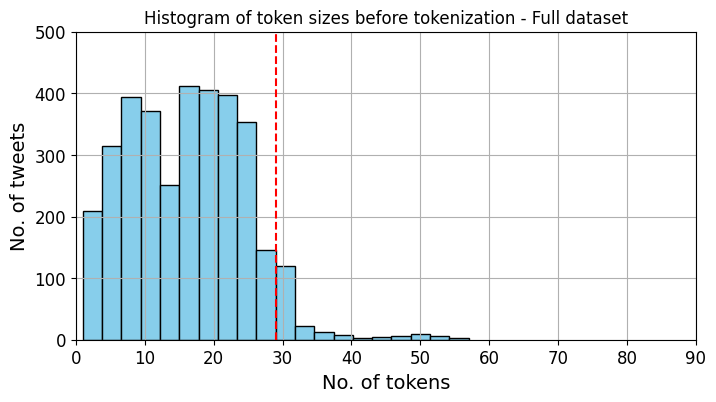
\includegraphics[width=0.5\textwidth]{figures/token_hist.png} % Replace with your image file name
    \caption{A sample figure caption.}
    \label{fig:sample}
\end{figure}
\section{Nested cross validation}
** To UPDATE **

\section{Domain splits with nested cross validation}
** To UPDATE **

\section{Ethical, Professional and Legal Issues}
** TO UPDATE **
